% Makros zur Kompatibilitaet mit Onlinemodul: 
 \providecommand{\MoIl}[1][]{\mbox{}#1]\mathopen{}} 
 \providecommand{\MoIr}[1][]{#1[\mbox{}} 
 \providecommand{\MIntvlSep}{;} 
 \providecommand{\MElSetSep}{\, ; \, } 
 \begin{MAufgabe}{Lineare Betrags(un)gleichungen}{vr, 2016, MaTeX}
L\"osen Sie die Gleichung
$$
 \MDS \left| 4\, x - 3 \right|+2\, x + 4= 3 \left| 4 - 4\, x \right| -4
$$  

\ifLsg\MLoesung

Im ersten Schritt k\"onnen die Terme au\ss{}erhalb der Betragszeichen zusammengefasst werden:

\begin{align*} 
 \left| 4\, x - 3 \right|+2\, x + 4= 3 \left| 4 - 4\, x \right| -4\\ 
\Leftrightarrow2\, x + \left|4\, x - 3\right| - 3\, \left|4\, x - 4\right| + 8= 0 
 \end{align*}

F\"ur diese Gleichung haben wir 4 F\"alle zu unterscheiden: 
\begin{enumerate}
\item $ \MDS 
\begin{cases} 
 0 \leq 4\, x - 3\\ 
0 \leq 4 - 4\, x
 \end{cases}
\Leftrightarrow x \leq 1 \wedge \frac{3}{4} \leq x\Leftrightarrow x \in [ \frac{3}{4} \, \MIntvlSep \, 1]$ 
\item $ \MDS 
\begin{cases} 
 0 \leq 4\, x - 3\\ 
4 - 4\, x < 0
 \end{cases}
\Leftrightarrow 1 < x\Leftrightarrow x \in \MoIl  1 \, \MIntvlSep \, \infty\MoIr $ 
\item $ \MDS 
\begin{cases} 
 4\, x - 3 < 0\\ 
0 \leq 4 - 4\, x
 \end{cases}
\Leftrightarrow x < \frac{3}{4}\Leftrightarrow x \in \MoIl  -\infty \, \MIntvlSep \, \frac{3}{4}\MoIr $ 
\item $ \MDS 
\begin{cases} 
 4\, x - 3 < 0\\ 
4 - 4\, x < 0
 \end{cases}
 \mbox{ : keine L\"osung. Diese Bedingung ist nirgendwo erf\"ullt.}$ 
\end{enumerate} 
Der 4. Fall ist nirgendwo erf\"ullt. Betrachte weiter nur die restlichen F\"alle.
 
 Fallunterscheidung: 

 \begin{enumerate} 
 \item Sei $ \MDS x\in[ \frac{3}{4} \, \MIntvlSep \, 1]$. 
 In diesem Fall gilt: 
  $ \MDS \left| 4\, x - 3\right|=4\, x - 3$ und $ \MDS \left| 4 - 4\, x\right|=4 - 4\, x$. \\ 
 Damit ist die Gleichung 
 $$ 
2\, x + \left|4\, x - 3\right| - 3\, \left|4\, x - 4\right| + 8= 0
$$
 \"aquivalent zur Gleichung
 $$ 
\left(4\, x - 3\right)-3\left( 4 - 4\, x\right)+2\, x+8= 0 
$$  
$$ 
 \Leftrightarrow 18\, x - 7= 0 
$$  
$$ \Leftrightarrow x = \frac{7}{18} . 
 $$ 
 Die L\"osung muss auch die Fallbedingung $x\in [ \frac{3}{4} \, \MIntvlSep \, 1] $ erf\"ullen. Die gefundene L\"osung $x=\frac{7}{18}$ erf\"ullt die Fallbedingung  $x\in [ \frac{3}{4} \, \MIntvlSep \, 1]$ nicht und deshalb ist  $$
 \mathcal{L}_{1}=\emptyset 
 $$ 
\item Sei $ \MDS x\in\MoIl  1 \, \MIntvlSep \, \infty\MoIr $. 
 In diesem Fall gilt: 
  $ \MDS \left| 4\, x - 3\right|=4\, x - 3$ und $ \MDS \left| 4 - 4\, x\right|=4\, x - 4$. \\ 
 Damit ist die Gleichung 
 $$ 
2\, x + \left|4\, x - 3\right| - 3\, \left|4\, x - 4\right| + 8= 0
$$
 \"aquivalent zur Gleichung
 $$ 
\left(4\, x - 3\right)-3\left( 4\, x - 4\right)+2\, x+8= 0 
$$  
$$ 
 \Leftrightarrow 17 - 6\, x= 0 
$$  
$$ \Leftrightarrow x = \frac{17}{6} . 
 $$ 
 Die L\"osung muss auch die Fallbedingung $x\in \MoIl  1 \, \MIntvlSep \, \infty\MoIr  $ erf\"ullen. Die gefundene L\"osung $x=\frac{17}{6}$ erf\"ullt die Fallbedingung  $x\in \MoIl  1 \, \MIntvlSep \, \infty\MoIr $ und deshalb ist  $$
 \mathcal{L}_{2}=\left\{\frac{17}{6}\right\}
 $$ 
\item Sei $ \MDS x\in\MoIl  -\infty \, \MIntvlSep \, \frac{3}{4}\MoIr $. 
 In diesem Fall gilt: 
  $ \MDS \left| 4\, x - 3\right|=3 - 4\, x$ und $ \MDS \left| 4 - 4\, x\right|=4 - 4\, x$. \\ 
 Damit ist die Gleichung 
 $$ 
2\, x + \left|4\, x - 3\right| - 3\, \left|4\, x - 4\right| + 8= 0
$$
 \"aquivalent zur Gleichung
 $$ 
\left(3 - 4\, x\right)-3\left( 4 - 4\, x\right)+2\, x+8= 0 
$$  
$$ 
 \Leftrightarrow 10\, x - 1= 0 
$$  
$$ \Leftrightarrow x = \frac{1}{10} . 
 $$ 
 Die L\"osung muss auch die Fallbedingung $x\in \MoIl  -\infty \, \MIntvlSep \, \frac{3}{4}\MoIr  $ erf\"ullen. Die gefundene L\"osung $x=\frac{1}{10}$ erf\"ullt die Fallbedingung  $x\in \MoIl  -\infty \, \MIntvlSep \, \frac{3}{4}\MoIr $ und deshalb ist  $$
 \mathcal{L}_{3}=\left\{\frac{1}{10}\right\}
 $$ 
 \end{enumerate} 
  Die L\"osungsmenge des Ausgangsproblems ist die Vereinigung der einzelnen L\"osungsmengen: 
$$ \mathcal{L} = \mathcal{L}_{1} \cup \mathcal{L}_{2} \cup \mathcal{L}_{3} 
 = \emptyset\cup \left\{\frac{17}{6}\right\}\cup \left\{\frac{1}{10}\right\} 
  =\left\{\frac{17}{6}\right\}\cup\left\{\frac{1}{10}\right\} 
  = \left\{\frac{17}{6}\MElSetSep\frac{1}{10}\right\} 
 . $$ 
 
 \begin{center}
 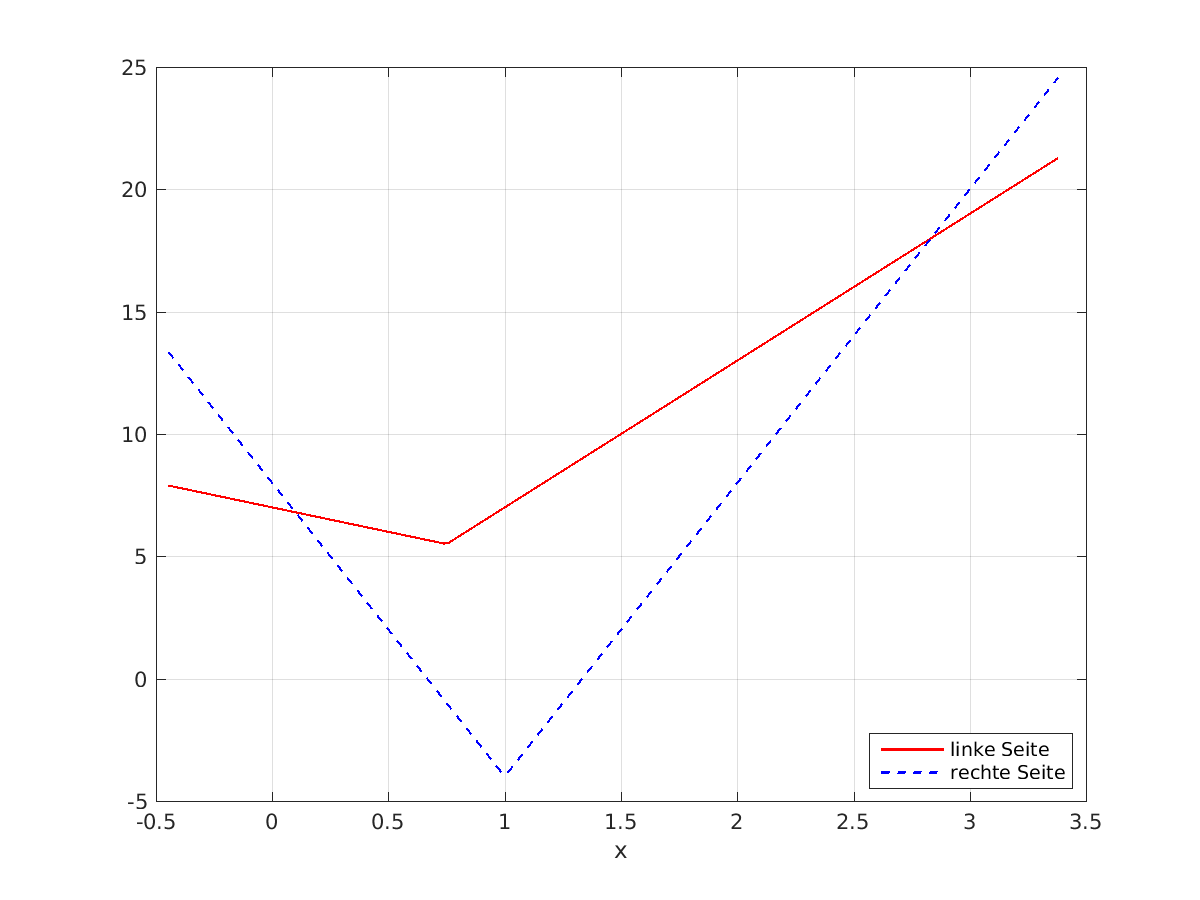
\includegraphics[width=0.8\linewidth]{Abb_zur_Ag_autogenerated_ineq_5.png} \end{center}
 
\else\relax\fi
 \end{MAufgabe}